\section{Architecture Integration}

\subsection{Model Support}

\begin{table}[H]
\centering
\small
\begin{tabular}{lllll}
\toprule
\textbf{Model} & \textbf{Attention path} & \textbf{Nested?} & \textbf{RoPE?} & \textbf{GQA?} \\
\midrule
DistilBERT & \texttt{layer[i].attention} & No & No & No \\
RoBERTa & \texttt{layer[i].attention.self} & Yes & No & No \\
GPT-2 & \texttt{h[i].attn} & No & No & No \\
Qwen3.5 & \texttt{layers[i].self\_attn} & No & Yes & Yes \\
\bottomrule
\end{tabular}
\end{table}

\subsection{Weight Transfer}

The \texttt{copy\_weights} procedure handles four patterns, delegated to the two 
branch modules:

\subsubsection{DistilBERT}

\begin{lstlisting}
q\_w = src.q\_lin.weight  # (768, 768)
k\_w = src.k\_lin.weight
v\_w = src.v\_lin.weight
o\_w = src.out\_lin.weight
\end{lstlisting}

\subsubsection{RoBERTa Nested}

\begin{lstlisting}
q\_w = src.self.query.weight
k\_w = src.self.key.weight
v\_w = src.self.value.weight
o\_w = src.output.dense.weight
\end{lstlisting}

\subsubsection{GPT-2 Conv1D}

\begin{lstlisting}
c\_w = src.c\_attn.weight.t()  # transpose
q\_w, k\_w, v\_w = c\_w.chunk(3, dim=0)
o\_w = src.c\_proj.weight.t()
\end{lstlisting}

\subsubsection{Qwen3.5 GQA}

\begin{lstlisting}
q\_w = src.q\_proj.weight  # (H d\_h, d)
k\_w = src.k\_proj.weight  # (H\_kv d\_h, d)
v\_w = src.v\_proj.weight
o\_w = src.o\_proj.weight
\end{lstlisting}

\subsection{The `out\_proj` Search}

The output projection is extracted using a search over candidate attributes:

\begin{lstlisting}
for cand in ("out\_proj", "out\_lin", "o\_proj", "output", "proj", "c\_proj", "dense"):
    for target in (old\_attn, old\_attn.self, old\_attn.attention, old\_attn.output):
        if target and hasattr(target, cand):
            ...
\end{lstlisting}

If no output projection is found, we \textbf{raise RuntimeError} to prevent 
injecting a random-init projection.

\subsection{Injection Algorithm}

\textbf{Algorithm 2:} Inject HGRN2-GatedDeltaNet into a full model
\begin{lstlisting}
Input:  model M, config c, lora\_rank, lora\_alpha
Output: M with attention replaced

1: layer\_list $\leftarrow$ find\_transformer\_layers(M)
2: for i, layer in enumerate(layer\_list) do
3:     src $\leftarrow$ extract\_attention(layer)
4:     if src is None or is\_already\_injected(src): continue
5:     try:
6:         new $\leftarrow$ HGRN2GatedDeltaNet(c, old\_attn=src, ...)
7:         replace(layer, new)
8:     except Exception as e:
9:         log\_warning(f"Layer {i} failed: {e}")
10:        continue
11: end for
12: return M
\end{lstlisting}

\subsection{The `sub\_kwargs` Pattern}

To avoid the "multiple values for keyword argument" error, we filter 
\texttt{kwargs} before passing to sub-branches:

\begin{lstlisting}
sub\_kwargs = {k: v for k, v in kwargs.items() 
              if k not in ("is\_decoder", "is\_causal", "lora\_rank", "lora\_alpha")}
\end{lstlisting}

This is essential when the same \texttt{kwargs} dict is passed through multiple 
levels of the call hierarchy.

\subsection{Causal Detection}

\begin{lstlisting}
\_decoder\_prefixes = ("gpt", "qwen", "llama", "mistral", "gemma", "phi", 
                     "opt", "bloom", "falcon")
if any(model\_type.startswith(p) for p in \_decoder\_prefixes):
    is\_dec = True
\end{lstlisting}

The flag is passed to both branches, which use it to switch between 
causal and bidirectional recurrences.

\subsection{Double-Injection Guard}

The injection function checks whether the target already contains a 
\texttt{HGRN2GatedDeltaNet}:

\begin{lstlisting}
if isinstance(curr\_attn, HGRN2GatedDeltaNet): return None
if "HGRN2GatedDeltaNet" in curr\_attn.\_\_class\_\_.\_\_name\_\_: return None
if hasattr(curr\_attn, "inner") and isinstance(curr\_attn.inner, HGRN2GatedDeltaNet): return None
if hasattr(curr\_attn, "\_wrapped\_attention") and isinstance(curr\_attn.\_wrapped\_attention, HGRN2GatedDeltaNet): return None
\end{lstlisting}

This prevents accidentally wrapping the module twice.

\subsection{Skipping Hybrid Layers (Qwen3.5)}

Qwen3.5 has some layers using \texttt{DeltaNet} or \texttt{LinearAttention}. We skip them:

\begin{lstlisting}
if "DeltaNet" in c\_name or "LinearAttention" in c\_name:
    return None
\end{lstlisting}

\subsection{Failure Modes}

\begin{lstlisting}

---
\end{lstlisting}

\begin{figure}[H]
\centering
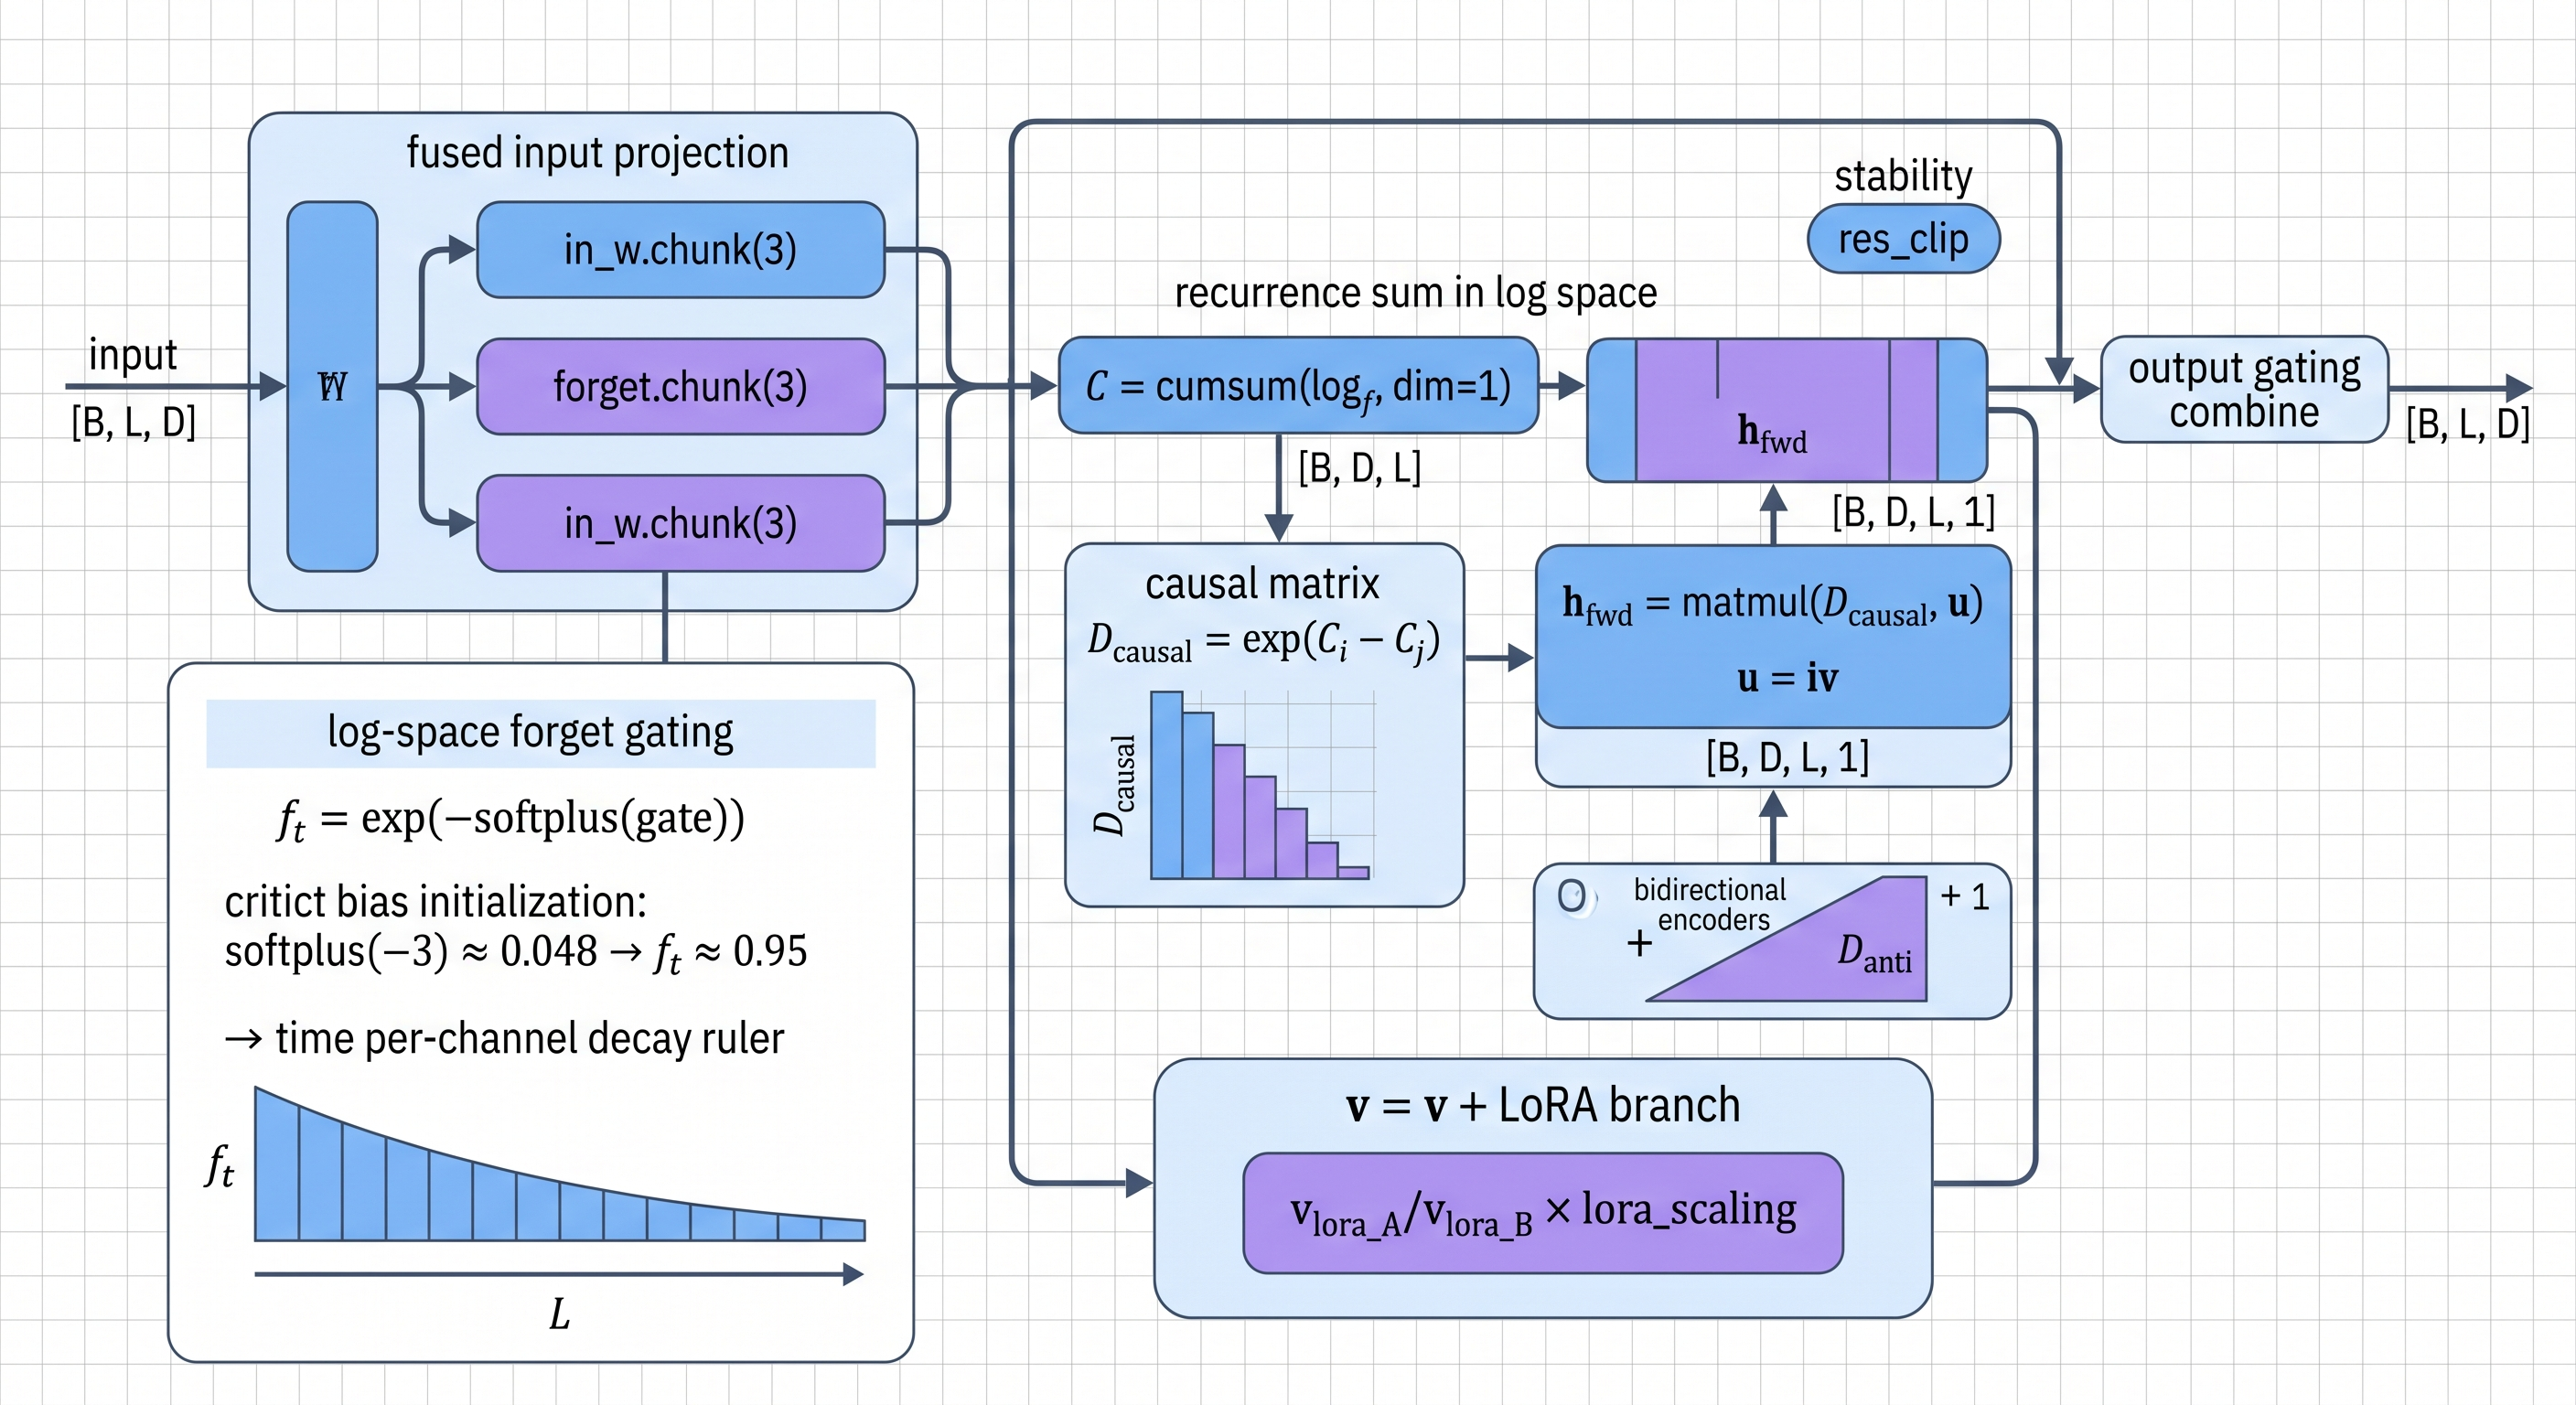
\includegraphics[width=\linewidth]{figures/architecture.jpeg}
\caption{High-level architectural diagram of hgrn2\_gated\_deltanet.}
\label{fig:arch_hgrn2-gated-deltanet}
\end{figure}

